

\begin{figure*}[!ht]
    \centering
    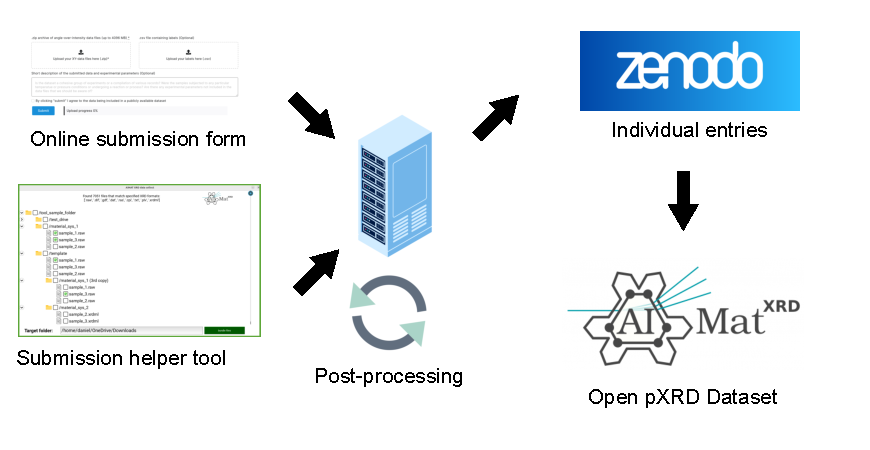
\includegraphics{figures/overview.pdf}
    \caption{Overview of the data collection pipeline. Datasets are submitted using an online submission form or our submission helper software. After post-processing and data homogenization, we create a Zenodo entry for each user submission and subsequently include the submission in the opXRD database.}
    \label{fig:overview}
\end{figure*}

% High throughput experimentation
The advent of high-throughput experiments holds the prospect of significantly accelerating the speed of materials discovery. \cite{Liu2019}
The synthesis and characterization of novel materials is becoming increasingly efficient and automated,
increasing the throughput of samples in experimentation pipelines. \cite{MacLeod2019, Ludwig2019, Ozaki2020}

% On Rietveld refinement
After fabricating a new material, a number of analysis techniques can be used to characterize the sample.
The most important method to determine the crystal structure of a new material is powder X-ray diffraction. 
To analyze pXRD data, an initial guess is optimized using Rietveld refinement. In this process, an initial crystal structure including unit cell parameters is provided by the operator of the analysis software and fitted to the observed diffractogram in an iterative optimization process based on simulated forward prediction of expected pXRD diffractograms given the current crystal structure.\cite{Dinnebier2019, Cano2021}
As Rietveld refinement is a local optimization method, the result of the refinement procedure is generally only as good as the initial guess it was provided with.
Therefore, it strongly relies on the experience of the operator to provide an accurate initial guess of the crystal structure.

Employing manually operated Rietveld refinement, including determining a good initial structure for the optimization, is not without issues.
It is certainly not scalable to the degree required to keep up with advances in throughput and efficiency in other steps of the experimentation pipeline.
Automation of the Rietveld refinement requires the automation of finding initial guess structures, which is highly non-trivial, and the automation of the iterative optimization procedure, which can be done using black-box optimization algorithms. \cite{Ozaki2020} 
Initial guesses for Rietveld refinement are often obtained by matching the observed diffractogram to patterns from a database.
However, for novel observed structure types, simply matching to a database of known structures will not yield good results. Therefore, more complex crystal structure solution approaches need to be applied to find suitable crystal structure guesses.

Machine learning has the potential to speed up the manual analysis of powder diffractograms and keep pace with an automated high-throughput experimentation environment. \cite{Agrawal2019, Surdu2023}
Models can be trained to predict crystal structure information directly given a diffractogram, or models can be used to automate the conventional workflow of finding an initial guess and running ML-automated Rietveld refinement. \cite{Surdu2023}    \cite{Feng2019} 
%However, the current limiting factor is the availability of sufficiently large labeled datasets.
So far, however, due to an absence of labeled datasets with experimental diffractograms, machine learning in this domain has largely relied on diffractograms simulated from known structures (such as from the ICSD) or, most recently, from generated synthetic crystals.

Models trained on datasets with simulated diffractograms have already shown very strong performance in predicting
lattice parameters, spacegroup, and crystallite size from simulated diffractograms.
However, the performance substantially drops off when these models are applied to data originating from experiments [cite 2-3 papers, incl. ours].
The patterns observed in experiments suffer from a host of imperfections that need to be modeled accurately in order to be able to transfer models trained on simulated data to experimental patterns. This includes noise, background, preferred orientation of the sample, ...
Most approaches currently model these imperfections as a simple signal based on a heuristic functional form added to the simulated diffractograms.

At the moment, the number of openly available datasets for experimental powder data is very limited.
The main sources for experimental patterns are XXX, YYY, and ZZZ.
Further commercial datasets such as KKK and LLL exist, but license fees and restrictions in their use to train publishable models or even publish the training data limit their usability.
Collecting a labeled dataset of raw experimental powder X-ray diffraction data of sufficient size to directly train a model that predicts crystal structure information is likely out of reach.
The most advanced ML models currently are trained on approximately $10^7 - 10^8$ simulated diffractograms, which is x orders of magnitude higher than the largest currently curated experimental dataset and x orders of magnitude larger than the opXRD dataset we present here.

However, even small labeled and also unlabeled experimental diffractograms hold significant value in practice. First of all, labeled data can be used to better test and benchmark existing and new automated analysis approaches, which yields a better comparison than when using the very limited currently available datasets, such as the commonly used RRUFF mineral dataset.

Furthermore, even completely unlabeled data can enable machine learning researchers to evaluate how closely their simulations represent actual experimental data, identify what features are missing, and modify their simulation algorithms accordingly to arrive at a simulation that mirrors how data appears in reality.
One can bring the simulated patterns closer to experiment by improving the simulation itself by properly modeling more of the observed physical effects such as preferred orientation, peak shapes resulting from different sources, etc.
Additionally, some of the observed imperfections, such as background and noise, can be modeled using machine learning approaches.
This is similar to the concept of style transfer\cite{Gatys2016, Ganin2015} found in the domain of machine learning applied to images.
Here, the objective is to obtain a classification or regression model when only labeled images of one style (simulated data) and unlabeled or partially labeled images of another style (experimental data) are available.

In this publication, we provide a new open powder X-ray diffraction (opXRD) dataset that collects a broad range of patterns from experiment, exceeding the currently available amount of openly accessible experimental patterns by XX.
Our opXRD dataset has been curated by collecting the accumulated powder data from multiple large research groups and institutions with high-throughput XRD facilities. It contains pXRD patterns from single and multiphase materials from a wide variety of materials classes, including XXX, YYY, and ZZZ. Details about the experiments of contributing research groups are discussed in this paper, along with a detailed description of how to contribute further data and how to use the data.

% How to contribute? This aspect deserves a separate paragraph
The opXRD database is planned as a growing, community-driven initiative. The dataset we present here is the first version, but we hope to further increase the dataset size through active engagement with the pXRD community. Our primary objective is to minimize the effort and thus the barrier to contributing experimental data to the opXRD database. Thus, we developed a program that helps to find and share data from e.g. pXRD lab computers. In detail, users can select their most common pXRD file types, the program lists all files of that type, and users can select or deselect certain folders or files for sharing. Selected contributions will be uploaded to opXRD, processed to a common file format, and - if wanted - published on Zenodo on behalf of the contributors, before becoming part of the opXRD database. If labels are available, they can be shared with opXRD as well. Further details can be found on the opXRD website (Figure~\ref{fig:overview}).

The broad range of available experimental samples contained in the opXRD v1.0 database makes it possible to apply state-of-the-art ML approaches to the domain of powder XRD analysis.
We hope that this will yield more advanced automated ML approaches in the future, which can readily be applied in high-throughput experimentation pipelines.


%-----------------------------------------------------------%
% Sources on rietveld refinement

% Computationally intensive -> Probably outdated. If it used to take minutes in 2010
% it probably only takes seconds by now.
% https://www.rigaku.com/de/node/707

% A simple solution to the Rietveld refinement recipe problem
% -> Rietveld refinement requires "expert input"
% https://www.ncbi.nlm.nih.gov/pmc/articles/PMC10840306/

% Comments -> Why having to do rietveld refinement sucks
% FullProf tutorial on fitting XRD peaks -> Tedious, requires lots of manual input
% https://pranabdas.github.io/research/fullprof/

% Topas tutorial -> 44 page tutorial, many boring and potentially frustrating steps, lots of points offer potential for task failure
% https://topas.webspace.durham.ac.uk/topas_user_menu/

%  Methods and Tutorials – Powder Diffraction -> Overview of rietveld refinement data
%https://neutrons.ornl.gov/sites/default/files/Methods%20and%20Tutorials%20Powder%20Diffraction.pdf

% Rietveld Refinement from Powder Diffraction Data -> 50 pg tutorial that no one wants to read, overwhelming amout of quantities/figures that needs to be manually looked at in the process
% https://www.fkf.mpg.de/4112052/cpd26.pdf